\chapter{Fejlesztői dokumentáció}

Egy integrált fejlesztői környezetnél többféle igény is megfogalmazható. Valamelyik fejlesztőnek
olyanra van szüksége, amely ugyan kevesebbet tud, de gyorsabban indítható, esetlegesen gyorsabban
végezhető vele a munka. SQL-hez található több integrált fejlesztői környezet, ilyen az Oracle-nél
például az SQL Developer\cite{sqldeveloper}.
Az én programom az SQL Developerhez képest kevesebb komponenst tartalmaz, így gyorsabb is. Tökéletes
eszköz, ha valaki csak a lekérdezésekre próbál koncentrálni.

A megvalósított programban lehetőség van...
\begin{itemize}
  \item Oracle adatbázishoz való kapcsolódáshoz,
  \item kapcsolat adatainak mentésére,
  \item ezen kapcsolati adatok törlésére,
  \item PL/SQL szkriptek végrehajtására,
  \item SQL lekérdezések végrehajtására,
  \item adatbázis objektumok megtekintésére, törlésére,
  \item lekérdezési tervek létrehozására,
  \item kör, illetve oszlopdiagramok készítésére.
\end{itemize}

A fejlesztéshez szükséges eszközök kiválasztásnál tehát szempont volt a hatékonyság, valamint hogy
ennek ellenére többet nyújtson az eddig elérhető programoknál, ezért esett a választásom a Qt-ra, ami egy C++ keretrendszer.
Nem csak hatékony kódot lehet vele készíteni, szükség esetén magas absztrakció is használható, és nem
csak egy operáció rendszeren fordítható a Qt-ban készített programok. Ezen felül elvárás hogy legyen intuitív kezelőfelülete,
és biztonságosan működjön.

\section{Fogalmak}
Itt részleteznék néhány fogalmat amivel jobb tisztában lenni mielőtt tovább olvasná a dokumentációt.

SQL egy lekérdezésekre megfogalmazására specializálódott nyelv, azaz egy szakterület-specifikus nyelv.
PL/SQL az Oracle által az SQL kiterjesztéseként kifejlesztett procedurális programozási nyelv. Továbbá egy host nyelv,
amin belül bizonyos kódrészleteket SQL segítségével írhatunk meg. Ezen fogalmak mélyebb ismerete ajánlott a továbbiakban.
Névtelen függvény egy helyben létrehozott és (akár) meghívott függvény.

\section{Megoldási terv}

\begin{figure}[ht]
  \begin{center}
  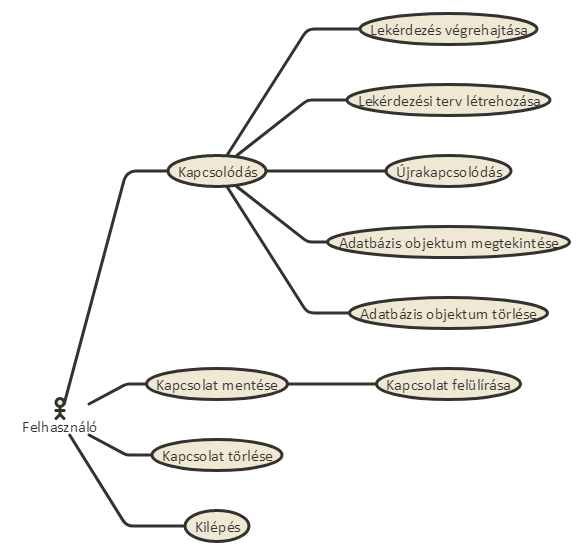
\includegraphics[max width=\textwidth]{usecase}
  \end{center}
 \caption{Felhasználói esetek}
\end{figure}

Felhasználóknak ezen felül lehetősége nyílhat más funkciók használatára is,
ám ezek a legfontosabbak, így ezeknek az implementálása az elsődleges.
Ezeknek az implementálása két külön ablakban történt a gyorsabb elérhetőség, és
a modularitás miatt: így bármikor lehetőség nyílik új ablak nyitására, esetleg
ha valaki akar felhasználhatja a programot és kódbol csatlakozhat az adatbázishoz.
Biztonsági szempontból ez nem ajánlatos, de ez is egy lehetőség ha nincs a számítógépen
biztonsági kockázat (pl. belső hálózatról működik csak, illetéktelen felhasználó nem férhet hozzá).

\subsection{Felhasználói felület terve}
\begin{figure}[ht]
  \begin{center}
  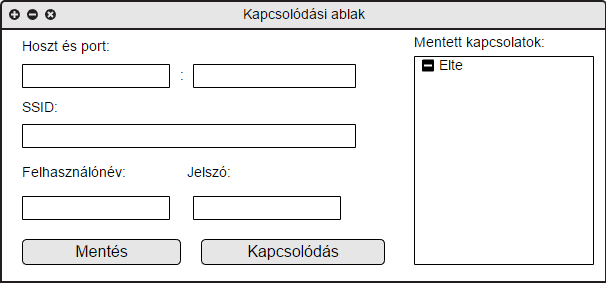
\includegraphics[max width=\textwidth]{connectionWindow}
  \end{center}
 \caption{Kapcsolódási ablak terve}
\end{figure}

A kapcsolódási ablaknál szempont volt az egyszerűség és könnyen kezelhetőség. Első használat
során már el lehet igazodni rajta bárkinek. Implementálás során fontos megjegyezni néhány szempontot
amit érdemes figyelmbe venni: a tabok sorrendje legyen meghatározott - balról jobbra, fentről lefele haladjon -, valamint
a jelszó mező tartalmát ne lehessen látni. Továbbá adatbázishoz kapcsolódás esetén legyen minél hamarabb eltűntetve a
jelszó a memóriából. (Megjegyzés: C++ esetén vigyázni kell az optimalizálásra, fordítótol függően könnyen lehet hogy a nem használt értékadást
eltűnteti a fordító) A kapcsolatokat lehessen szerkeszteni, azaz lehessen felülírni. Erről jelenjen meg egy figyelmeztetés is,
hogy véletlen se írja felül a felhasználó a korábbi kapcsolatát. Ezen felül ha bármilyen hiba (nem lehet fájlt/mappát megnyitni, vagy létrehozni)
történik, akkor azt jelezze a program ennek megfelelően. Kapcsolat törlése esetén is kérjen megerősítést a program.

\begin{figure}[ht]
  \begin{center}
  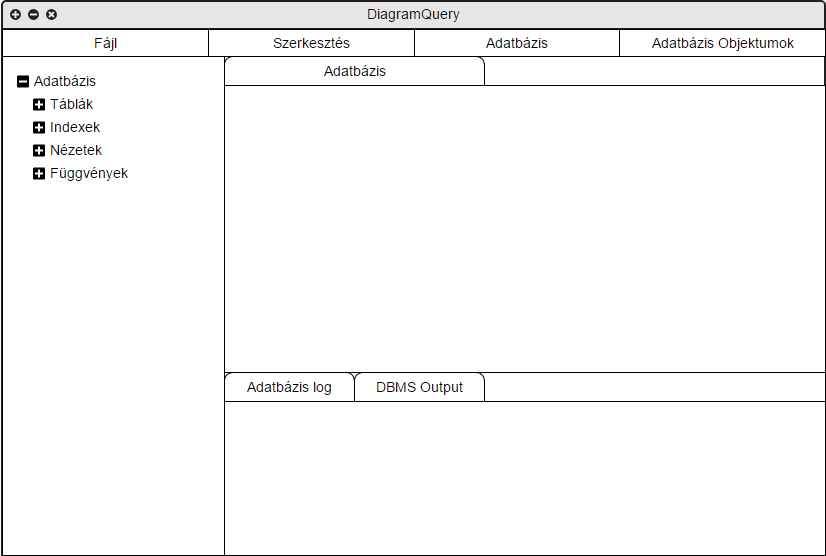
\includegraphics[max width=\textwidth]{mainWindow}
  \end{center}
 \caption{Fő ablak terve}
\end{figure}

A kapcsolódás után fogadja a felhasználókat a fő ablak. Legfontosabb itt, hogy a felhasználó rögtön munkához tudjon látni.
Érdemes úgy készíteni, hogy a képernyő nagy részét a szerkesztő tegye ki. Bal oldalon egy fában jelenjenek meg az adatbázis objektumai
(táblák, nézetek, függvények, indexek) és lehessen megtekinteni illetve törölni őket. A képernyőn jelenjen meg egy logban a futási idő,
illetve ha hiba történik az legyen szemmel látható. PL/SQL szkriptek miatt érdemes egy külön lapon megjeleníteni a kiírt üzeneteket is.
Azonkívül legyen lehetőség a szerkesztő törlésére, mentésére, valamint már meglévő *.sql fájl betöltésére is. A program adjon figyelmeztetést
törlés esetén. Mindemelett lehessen újra kapcsolódni az adatbázishoz arra az esetre ha megszakadna a kapcsolat az adatbázissal, valamint
lehessen új kapcsolatot is nyitni, ami zárja be a jelenlegit. Legyen lehetőség az adatbázis objektumok megtekintésére és törlésére is.
A szerkesztőablakba beírt SQL lekérdezések, PL/SQL szkriptek, illetve egyedi parancsok (diagramok készítésére) hajtódjanak végre megfelelően,
és legyen látható pontosan mit hajtott végre a program. A szerkesztő betűtípusa legyen jól olvasható, a tabulátor mérete alapértelmezetten legyen
4, illetve az SQL és PL/SQL kulcsszavak legyenek kiemelve.

\subsection{Komponensek}

\begin{figure}[ht]
  \begin{center}
  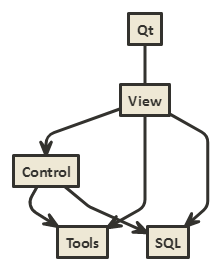
\includegraphics[scale=0.5]{components}
  \end{center}
 \caption{Komponensek}
\end{figure}

A program négy fő komponensből áll: Control, View, SQL, Tools. Mindegyik komponense a programnak külön felhasználható,
valamint bővíthetőek. Az SQL komponens azonban főként Oracle SQL-hez lett írva, így nem feltétlen működik minden
SQL variánsal, de ez később bővíthető. Az osztályokon kívűl egyéb függvényeket is tartalmaznak ezen komponensek, valamint
konstansokat is: ezek a jobb érthetőség és átláthatóság miatt kerültek legfőképp a programba.

\subsubsection{Control}

\begin{figure}[ht]
  \begin{center}
  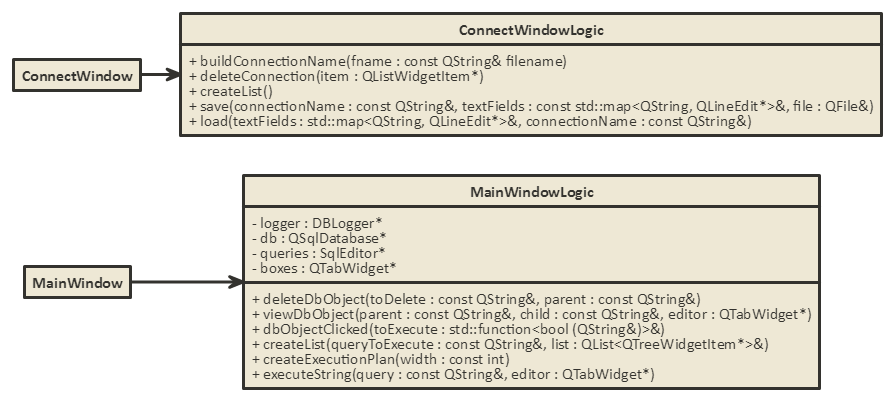
\includegraphics[max width=\textwidth]{control}
  \end{center}
 \caption{ Kapcsolódási- és főablak logikájának diagramja}
\end{figure}

Ebben a komponensben található a program logikája. Pontosabban itt, ebben a rétegben kerülnek a diagramok előállításra, valamint
itt kerülnek végrehajtásra a különböző lekérdezések. Miután a program végrehajtott egy utasítást, azután logolásra kerül a végrehajtás sikerettségét
jelző üzenet, valamint a hibaüzenet is sikertelen futás esetén.

\subsubsection{View}

\begin{figure}[ht]
  \begin{center}
  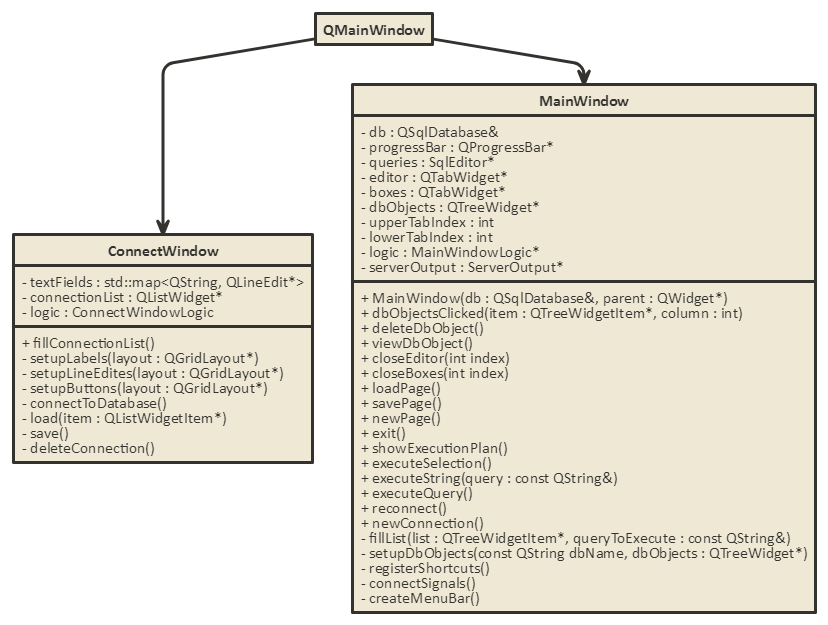
\includegraphics[max width=\textwidth]{view}
  \end{center}
 \caption{Kapcsolódási- és főablak diagramja}
\end{figure}

A View komponens felel a program kinézetéért. Itt van pontosan elrendezve minden nézetbeli elem, és itt vannak az események is lekezelve.
Fontos hogy jól érthető hibaüzeneteket jelenítsen meg ha valami nem rendeltetésszerűen történik, és ezt a felhasználó egyből észrevegye.
Későbbi szekcióban megtalálható a pontos terve a felhasználói felületnek, az alapján készítsük ezt el. A két legfontosabb függvény amit kiemelnék
a \textit{ConnectWindow::connectToDatabase()} és a \textit{MainWindow::reconnect()}.

ConnectWindow::connectToDatabase() metódus végzi el az adatbázishoz való kapcsolódást. Szüksége lesz az adatbázis, és a felhasználó adataira.
Az adatbázis adatai úgy mint a hoszt, port, serviceid (később esetlegesen a driver ami szükséges az adatbázishoz való kapcsolódáshoz). Valamint a 
felhasználó adatai úgy mint a neve és jelszava. A függvény írja ki ha hiba történik belépés során, illetve ha nem akkor csatlakozzon az adatbázishoz
és törölje a felhasználó jelszavát. Továbbá ez a metódus köti össze a kapcsolódási és főablakot.

A MainWindow::reconnect() metódus felelős a kapcsolat újboli kiépítésére. Bemenő adatai a felhasználó neve és jelszava. Abban az esetben ha a felhasználó
hibás adatokat ad meg, természetesen nem dobja el a régi kapcsolatot, hanem értesíti a felhasználót a hibáról. Megfelelő adatok esetén belépteti a felhasználót,
és az folytathatja tovább eddigi munkáját. Erre legfőképp azért lehet szükség, mert bizonyos adatbázis szerverek (pl. Oracle) egy idő után kidobják a felhasználót.
Ilyenkor az egész programot újra kéne indítani ha erre nem adnánk lehetőséget.

\subsubsection{SQL}

\begin{figure}[ht]
  \begin{center}
  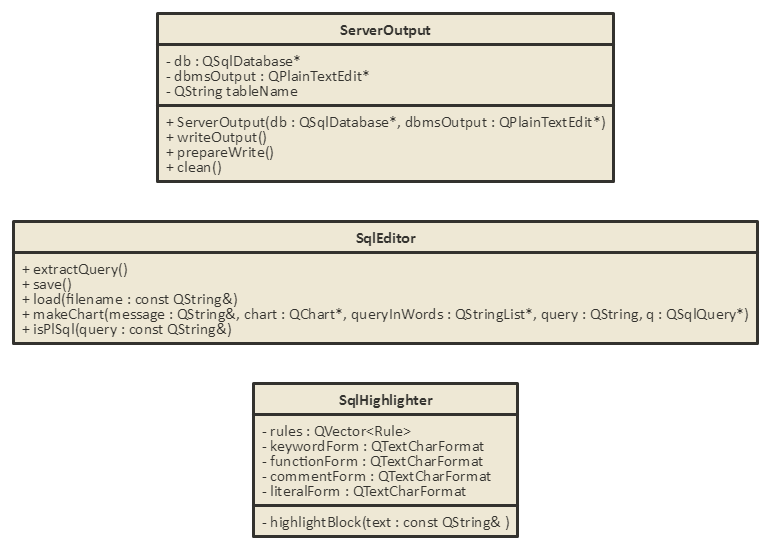
\includegraphics[max width=\textwidth]{sql}
  \end{center}
 \caption{SQL komponens osztályainak diagramja}
\end{figure}

Az SQL komponens végzi el a nyelvhez kapcsolódó feladatokat: szerkesztőfelülelet kialakítása, szintaxis kiemelése, a lekérdezések és szkriptek
megfelelő kiszedése. A cél az hogy akár önmagában is használható legyen (feltéve ha van egy adatbázis biztosítva hozzá), és minden SQL művelet
elvégezhető legyen a segítségével.

SQLHighlighter osztály reguláris nyelvtannal végzi el a kapott szöveg elemzését. Az összes SQL és PL/SQL kulcsszavak\cite{sqlwords} kiemelését
elvégzi, továbbá a kommenteket, szám- és szövegliterálokat is másképp emeli ki a könnyebb érthetőség kedvéért.
Ennek az osztálynak egy metódusa van, a \textit{highlightBlock()} aminek a bemenete egy szövegliterál. Ezt a bemeneti szöveget elemzi a metódus,
majd reguláris kifejezések segítségével kiemeli a kulcsszavakat, és literálokat a szabályoknak megfelelően.

ServerOutput osztály a DBMS\_OUTPUT kiírására szolgál. Egy temporáris táblába tárolja el a kiírt sorokat amit a bufferből olvas, majd ezt kérésre
kiírja, és törli. Külön osztály azért szükséges ehhez, hogy kilépés esetén törölje maga után a létrehozott temporáris objektumokat a program a
RAII elvei szerint. Egyetlen fontos metódusa a \textit{writeOutput()} aminek nincs bemenete és kimenete, csupán kiírja a megfelelő helyre a
buffer tartalmát.

Az SQLEditor osztály valósítja meg a fő szerkesztő felületét az osztálynak. Ezen felül ez az osztály hozza létre a diagramokat, és kezeli le az
esetlegesen hibás bemeneteket. A szerkesztéssel kapcsolatos logika is itt található: itt történik a végrehajtandó utasítások kiemelése (persze a
végrehajtásuk nem ebben az osztályban történik), a diagramok feldolgozása és kirajzolása, valamint a lapok mentése és betöltése is. Annak érdekében
hogy jobban hasonlítson eegy szerkesztőhöz, a jelenleg aktív sorokat is kiemeli, valamint ha futtatunk egy utasítást, vagy utasításokat, akkor azokat
is kiemeli hogy a felhasználó tisztában legyen azzal, hogy a program mit hajtott végre.

\subsubsection{Tools}

\begin{figure}[ht]
  \begin{center}
  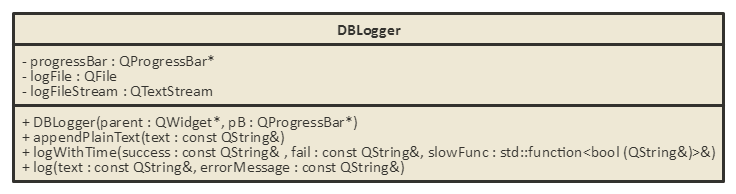
\includegraphics[max width=\textwidth]{tools}
  \end{center}
 \caption{Tools komponens osztályának diagramja}
\end{figure}



\section{Megvalósítás}
\subsection{Eszközválasztás}
\subsection{SQL eszközök}
\subsection{Felhasználói felület}
\subsection{Fejlesztői környezet}

\section{Továbbfejlesztési lehetőségek}

\section{Tesztelés}